



\section{Calibración}
\label{calibracion}

\subsection{Introducción}
Para poder obtener la posición en tres dimensiones de los marcadores a partir de las imágenes capturadas es necesario que las cámaras estén previamente calibradas. El objetivo de la calibración consiste en determinar un conjunto de parámetros tal que pueda establecerse una relación entre el espacio 3D y las coordenadas 2D de las imágenes.\\

Los puntos en el espacio pueden ubicarse respecto a un sistema de coordenadas 3D. A su vez, los puntos capturados en las imagenes pueden referenciarse respecto a un sistema de coordenadas 2D en píxeles. Si se quiere determinar la posición de un punto en el espacio en función de las correspondientes proyecciones de dicho punto en las imágenes capturadas por las cámaras, es necesario determinar las ecuaciones que vinculan al sistema de coordenadas del espacio con el sistema de coordenadas en píxeles de las cámaras.\\

De la relación entre estos sistemas de coordenadas se obtienen los parámetros de las cámaras. Dichos parámetros se clasifican en intrínsecos y extrínsecos. Los primeros son aquellos que describen las propiedades geométricas y ópticas de la cámara, es decir, las características internas de la cámara. Por otra parte, los parámetros extrínsecos son los que describen la posición y orientación de la cámara respecto al sistema de coordenadas del espacio.\\

Para realizar esto es necesario establecer un modelo que describa el sistema de óptico de las cámaras. Esto es, el modelo por el cual una cámara es capaz de transformar el espacio 3D en imágenes de dos dimensiones. Un modelo simple y que describe estos sistemas adecuadamente es el modelo \textit{pinhole} de las cámaras. 
El modelo \textit{pinhole} se basa en la implementación mas simple de una cámara real, la cámara estenopeica. En dicha cámara la imagen capturada esta conformada por la proyección del espacio 3D a través de un punto situado delante de la pantalla de la cámara como se muestra en la figura \ref{pinhole_camara}.\\

\begin{figure}[h!]
\begin{center}
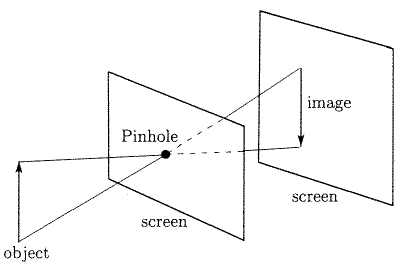
\includegraphics[scale=0.5]{img/calibracion/pinhole_camara.png}
\end{center}
\caption{Cámara estenopeica .\cite{faugueras_libro}}
\label{pinhole_camara}
\end{figure}


El modelo de esta cámara se describe en la figura \ref{pinhole_modelo}.\\

\begin{figure}[h!]
\begin{center}
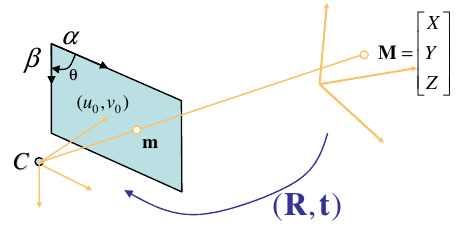
\includegraphics[scale=0.7]{img/calibracion/pinhole_modelo.png}
\end{center}
\caption{Modelo "pinhole" de una cámara.\cite{zhang_libro}}
\label{pinhole_modelo}
\end{figure}

En dicho modelo, una cámara se representa por un punto $C$, foco de la cámara, y un plano, al  que se le llama retina de la cámara. La imagen que se proyecta en la retina corresponde a la imagen capturada por la cámara. Dado un punto $M$ en el espacio, su correspondiente proyección en la retina, el punto $m$, se encuentra en la intersección de la retina y la recta formada por los puntos $C$ y $M$ de manera que $C$, $M$ y $m$ son colineales.\\ 



Si las coordenadas del punto  $M$ y las del punto $m$ son las siguientes:


\[m = \begin{bmatrix}
u \\ 
v
\end{bmatrix} , \quad
M = \begin{bmatrix}
X \\ 
Y \\
Z
\end{bmatrix} \]

Notando con $\tilde{x}$ a los vectores en coordenadas homogenes(anexo explicando esto?) se tiene:

\[\tilde{m} = \begin{bmatrix}
u \\ 
v \\
1
\end{bmatrix} , \quad
\tilde{M} = \begin{bmatrix}
X \\ 
Y \\
Z \\
1
\end{bmatrix} \]

Tomando el modelo \textit{pinhole} de la cámara, la relación entre un punto $M$ y su proyección $m$ es:
\begin{equation}
s\tilde{m} = A [R \quad t]\tilde{M}
\label{proyeccion}
\end{equation}




\begin{equation}
\text{siendo }
A = \begin{bmatrix}
\alpha & c & u_0 \\ 
0 & \beta & v_0 \\ 
0 & 0 & 1
\end{bmatrix} 
\end{equation}

Por lo tanto estos puntos se relacionan a través de la matriz $P = A [R \quad t]$, a menos de un factor de escala $s$. A dicha matriz  se le denomina Matriz de Proyección de la cámara.\\

La matriz $P$ se compone a su vez de la matriz $A$ que representa los parámetros intrínsecos de la cámara, y la matriz $[R \quad t]$ que representa los parámetros extrínsecos.\\

La matriz $[R \quad t]$ está formada por la rotación y traslación que relaciona el sistema de coordenadas del espacio con el sistema de coordenadas de la cámara. La matriz $A$ está formada por los parámetros intrínsecos de la cámara:\\



\begin{tabular}{cp{.8\textwidth}}


$(u_0, v_0)$ &  coordenadas del punto principal. \\ 
$\alpha$ y $\beta$ & factores de escala en los ejes de imagen  $u$ y $v$. \\ 
$c$ & grado de oblicuidad de los ejes imagen
\end{tabular} \\

El punto principal $(u_0, v_0)$ se define como el punto formado por la intersección de la retina y la recta perpendicular a dicha retina que pasa por el punto $C$. La distancia entre el punto $C$ y el punto principal se define como la distancia focal de la cámara $f$. Los factores $\alpha$ y $\beta$ se relacionan con la relación de aspecto de los píxeles de la cámara. El parámetro $c$ se relaciona con el ángulo $\theta$ formado por los ejes $u$ y $v$.\\

Por lo tanto la proyección de un punto 3D sobre la retina se compone de los siguientes pasos:\\

\begin{itemize}
\item Se pasa del sistema de coordenadas del espacio 3D $(X_w, Y_w, Z_w)$ al sistema de coordenadas de la cámara $(X,Y, Z)$
\begin{equation}
[X \ Y \ Z] = [X_w \ Y_w \ Z_w]^T + t
\end{equation}
\item Se proyecta el punto 3D respecto a las coordenadas de la cámara sobre las coordenadas imágen de la retina $(x,y)$.
\begin{equation}
x=f \dfrac{X}{Z} \qquad y = \dfrac{Y}{Z}
\end{equation}
\item En algunos casos puede ser necesario modelar además ciertas distorsiones introducidas por el lente de la cámara.
\begin{equation}
\check{x} = x + \delta_x \qquad \check{y} = y + \delta_y
\end{equation}

Siendo $(\check{x},\check{y})$ las coordenadas distorsionadas y $(\delta_x, \delta_y)$ las distorsiones aplicadas a $(x,y)$.

\item Por último se pasa de la coordenadas imagen $(\check{x}, \check{y})$ a las coordenadas en píxeles $(\check{u}, \check{v})$.

\begin{equation}
\check{u} + d_x ^{-1}\check{x} + u_0 \qquad \check{v} + d_y ^{-1}\check{y} + v_0
\end{equation}

Siendo $d_x$ y $d_y$ las distancias entre pixeles adyacentes en las direcciones horizontal y vertical, respectivamente.\\
\end{itemize}


\subsection{Métodos de calibración}

(referencia). De acuerdo a los objetos utilizados para realizar la calibración, los métodos pueden clasificarse de la siguiente manera.\\

\begin{itemize}
\item Calibración mediante objetos 3D\\

La calibración mediante este método es realizada capturando la imágen de un objeto de calibración cuyas dimensiones y geometría son conocidas. Los objetos de calibración suelen ser planos colocados otrogonalmente. También pueden utilizarse estructuras con marcadores de dimensiones conocidas.Estos objetos se le aplica traslaciones en el espacio logrando más cantidad de puntos de referencia para calibrar. La ventaja de este método es su precisión aunque se requiere de objetos más costosos y procedimientos más elaborados.\\

\item Calibración mediante objetos 2D\\

Este caso se utiliza objetos planos con figuras de patrones determinados, por ejemplo dameros. Estos objetos son colocados en varias posiciones delante de la cámara de manera de capturar varias imágenes del objeto. Esta metodología ofrece más flexibilidad para calibrar.\\

\item Autocalibración\\

Este método consiste en obtener la información necesaria a través de la captura de varias imágenes de un escena estática, prescindiendo de objetos para calibrar. Esta método es más flexible que  los anteriores aunque suele ser menos preciso.\\

\end{itemize}


Algunas soluciones comerciales, como por ejemplo Vicon \footnote{\textcolor{blue}{\underline{\url{www.vicon.com}}. Accedido 3-12-14.}} , utiliza como objeto de calibración una vara con leds, ver figura \ref{vicon}. 

\begin{figure}[H]
        \centering
        
        \subfloat{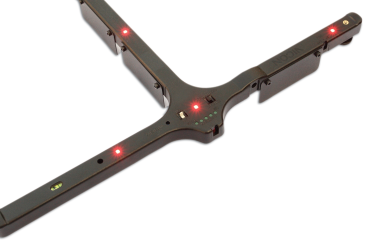
\includegraphics[scale=1.8]{img/calibracion/vicon1.png}\label{peladoOriginalintro}}
        \hspace{1.8cm}
        \subfloat{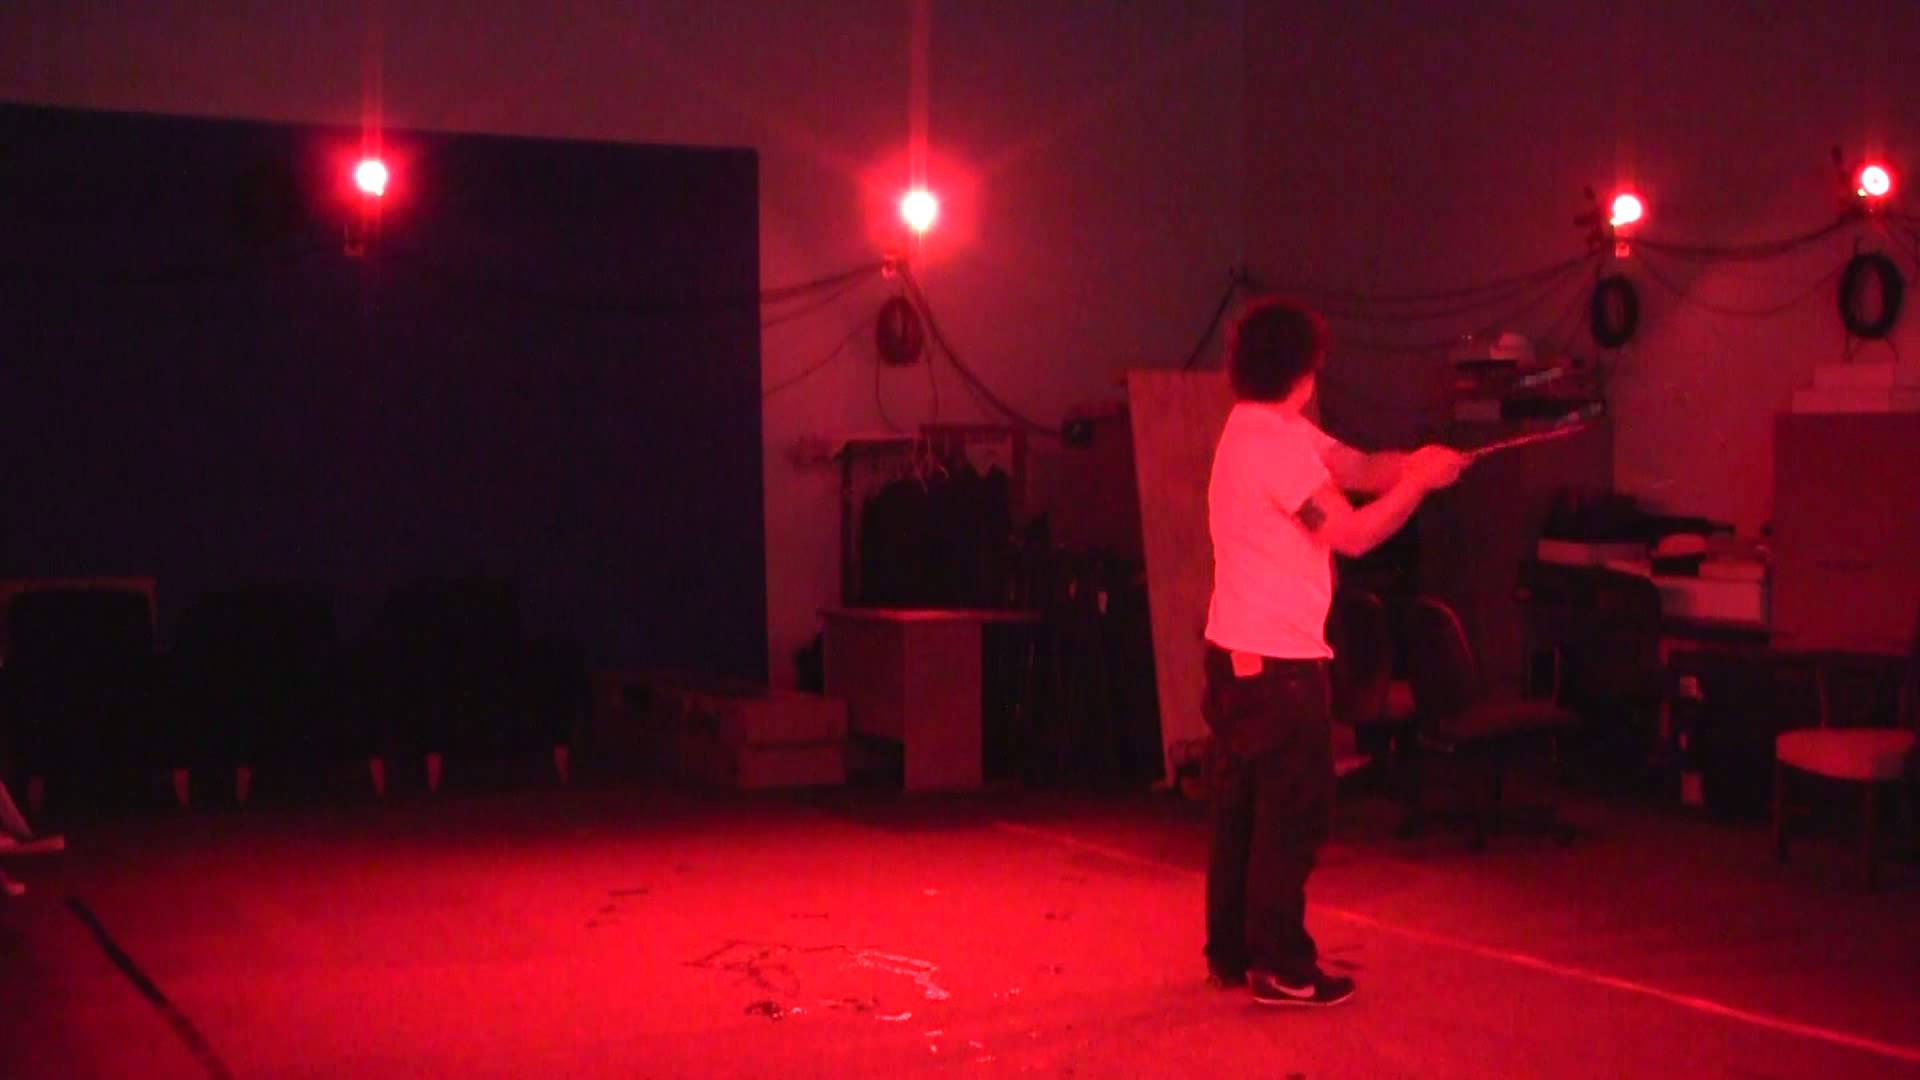
\includegraphics[scale=0.08]{img/calibracion/vicon2.jpg}\label{peladocirculosintro}}
  \caption{Calibración Vicon}
      \label{vicon}
\end{figure}

En este caso la calibración se realiza moviendo el objeto de calibración a través del espacio de trabajo. Este método resulta muy flexible para la calibración de un conjunto de varias cámaras simultáneamente.








